%%%%%%%%%%%%%%%%%%don't forget if needed %%%%%%%%%%%%%%%%%%%%%
%\section[toc version]{title version%
%              \sectionmark{head version}}
%\sectionmark{head version}
%%%%%%%%%%%%%%%%%%%%%%%%%%%%%%%%%%%%%%%%%%%%%%%%%%%%%%%%%%%%%%
\def\titcourt{Numerical simulation of phase change materials}
\def\titlong{Numerical simulation of phase change materials}
%%%%%%%%%%%%%%%%%%%%%%%%%%%%%%%%%%%%%%%%%%%%%%%%%%%%%%%%%%%%%%%%
\chapter[\titlong]{\titlong%
              \chaptermark{\titcourt}}
\chaptermark{\titcourt}
\label{chap-MELTING}
%%%%%%%%%%%%%%%%%%%%%%%%%%%%%%%%%%%%%%%%%%%%%%%%%%%%%%%%%%%%%%%%
%%%%%%%%%%%%%%%%%%%%%%%%%%%%%%%%%%%%%%%%%%%%%%%%%%%%%%%%%%%%%%%%

Having validated our code for the Navier-Stokes-Boussinesq solver, including both two-dimensional and three-dimensional problems,
we now pay a closer attention to phase-change systems evolving natural convection.
Two new non-linearities are considered in the system: the Carman-Kozeny penalty term and the enthalpy source term $S$.
The Carman-Kozeny penalty term is used to ensure zero velocity in the solid region since the same system of equations are
solved throughout the whole domain.
The enthalpy non-linear source term is used to model the phase-change in the energy equation.

Experimental and numerical benchmarks from the literature are used to validate our method.
The first part of this section is devoted to extensive validation and analysis of the octadecane PCM, generally use for buildings purposes,
due to its phase change temperature of $28^o C$.
Three benchmarks are considered: \cite{Okada1984} (experimental), \cite{gong2015numerical} (experimental) and \cite{bertrand1999melting} (numerical).
We provide then details about the time evolution of different physical parameter of the system.
The time evolution of the melting process is discussed first, in which the existence of three distinct regimes is drawn.
A comparison of the evolution of the Nusselt number and the liquid fraction with some analytical correlations is then given.
Finally, the influence of the Rayleigh number on the melting process is developed. 

Different geometries and materials are presented in a second part of this section to illustrate the capability of our method to deal with complexe configurations:
melting of cylindrical PCM with inner heated tubes, solid crust formation in a highly distorted mesh and melting of Gallium.

For the simulation of the melting process, we use the following choice for the scaling introduced in \S \ref{sec-eq-scaling}, equations (\ref{eq-adim}) and  (\ref{eq-RePr}):
\begin{equation}\label{ref-adimPCM}
V_{ref}=\frac{\nu_l}{H}  \, \Rightarrow  \, t = t_{\varphi}\frac{\nu_l}{H^2} \, \Rightarrow  \, \Rey  = 1. \\
\end{equation}
Moreover, a second dimensionless time $\tau$ is introduced in order to assess our results with respect to the numerical data of \cite{bertrand1999melting} and the analytical correlation of \cite{jany1988scaling}:
\begin{equation}
\label{eq-adim-tau}
\tau = \Ste\cdot Fo = \Ste\cdot \frac{\alpha t_{\varphi}}{H^2}  = \Ste\cdot \frac{t}{Pr},
\end{equation}
where $Fo$ is the Fourier number. 

We recall that the reference temperature is the fusion temperature and thus $\theta_f = 0$. The regularization range is defined for $ -\varepsilon_1 \leq \theta \leq \varepsilon_2 $, with $\varepsilon_1 = \varepsilon_2 = 0.01$.  
We also assume that physical properties of the material are identical in both liquid and solid phases, and, consequently, we obtain from (\ref{eq-adimKC}) that   $C(\theta)=1$ and $K(\theta)=1$.
This choice of the scaling was made to have the same set of parameters as in previous numerical simulations of this case \citep{Okada1984, Wang2010, Ma2006, dan-2014-JCP}. 

\section{Melting of octadecane PCM: numerical validation and physical analysis}\label{sec: melting-2D}
\subsection{Comparison with experimental data of \cite{Okada1984}  and \cite{gong2015numerical}, and numerical data of \cite{bertrand1999melting}.}

Three cases are investigated.
The first consists of an experimental study of the melting of the PCM in a differentially heated square cavity of height $H=1.5$ cm by \cite{Okada1984}.
The second reproduces the melting of the PCM included in a transparent building brick of height $H = 15.2$ cm, investigated experimentally and numerically by \cite{gong2015numerical}.
The last compares our results with various numerical methods, presented by \cite{bertrand1999melting}, simulating the melting of octadecane, considering a higher value of the Rayleigh number.\\
\begin{figure}
	\begin{center}
		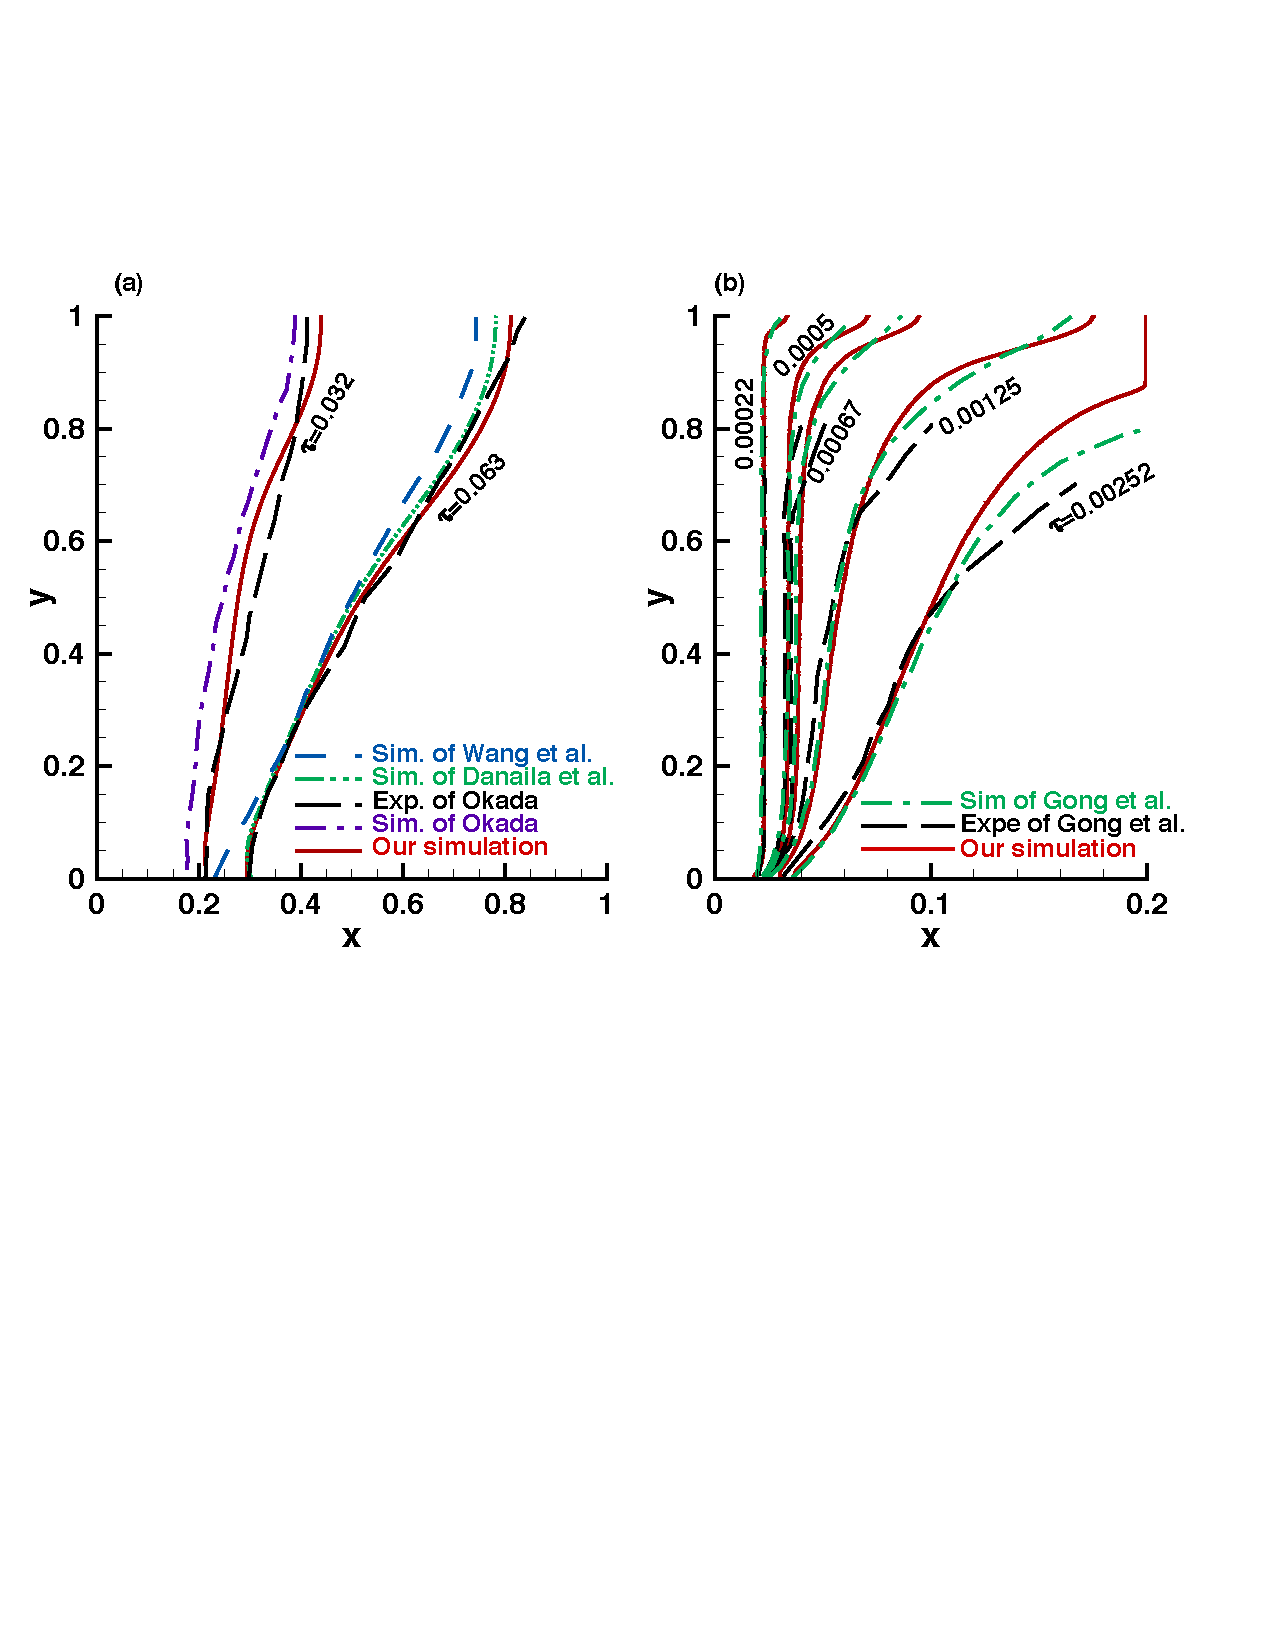
\includegraphics[width=0.85\textwidth]{\figpath/Fig_cap_melting/fig02_2}
	\end{center}
	\caption{Location of the interface during the melting of the PCM. 
	(a) Comparison with experimental data of \cite{Okada1984} and numerical results of \cite{dan-2014-JCP} and \cite{Wang2010} for two time instants ($\tau=0.032$ and $0.063$). Benchmark 1: $\Ray = 3.27 \cdot 10^5$, $\Pr = 56.2$ and $\Ste = 0.045$
	(b) Comparison with both experiment and simulation of \cite{gong2015numerical} for five time instants  ($\tau = 0.0002$, $0.00050$, $0.00067$, $0.00125$, $0.00252$). Benchmark 2: $\Ray = 2.48 \cdot 10^8$, $\Pr = 50$ and $\Ste = 0.072$.
	}
	\label{fig:pcm-valid}
\end{figure}

We first examine the location of the interface obtained in our simulations.
The comparison with the experimental results of \cite{Okada1984} and \cite{gong2015numerical} is presented in Figure \ref{fig:pcm-valid}.
The experimental study of \cite{Okada1984} in Figure \ref{fig:pcm-valid}(a) consists of a differentially heated square cavity of dimensions $1.5$ cm $\times \, 1.5$ cm, filled with an octadecane paraffin. The non-dimensional parameters are: $\Ray = 3.27 \cdot 10^5$, $\Pr = 56.2$ and $\Ste = 0.045$ (Benchmark 1).

For two particular time instants ($\tau=0.032$ and $\tau=0.063$), we could compare our results to available experimental \citep{Okada1984} and numerical \citep{Okada1984,Wang2010,dan-2014-JCP} data. 
In the experimental set up of \cite{Okada1984}, the author has reported that the top of the PCM was not perfectly insulated and consequently the growth of the experimental upper melting front was delayed.
In Figure \ref{fig:pcm-valid}(a), for the two time instants $\tau=0.032$ and $\tau=0.063$, the current work agrees well with the experimental results of \citep{Okada1984} at the bottom part of the melting front.
However, our results overestimate the location of the front in the top part of the cavity, which could be related to the experimental heat loss mentioned by the author.

Moreover, our results are qualitatively in a better agreement with experimental data than previously published numerical results. 
This is a direct consequence of the precise tracking of the melting front achieved by the mesh adaptivity performed at each time step. 
This assessment also allowed us to finely tune the value of the constants used in the model (\ref{eq-CK}). 
Even though it is generally assumed that a large value for $\CKC$ must be set, the exact value of this constant could influence the accuracy of the results \citep{kheirabadi2015effect, kumar2017influence}. 
This choice of the value of this constant is a still open problem.  
Very good agreement with the experimental result of \cite{Okada1984} is obtained for $\CKC$ varying in the range $[10^6, 10^8]$. 
Nevertheless, imposing  a too large value $\CKC=10^{10}$ results  in artificially slowing the propagation of the melting front. We set for all subsequent simulations $\CKC= 10^6$. \\

Figure \ref{fig:pcm-valid}(b) illustrates the interface location in the experiment and simulations of   \cite{gong2015numerical}, who studied the melting of an octadecane PCM inside a transparent building brick of dimensions 
$15.2$cm$\times 3$cm.
Their numerical simulation has been performed using a Lattice Boltzmann method. 
The non-dimensional parameters were: $\Ray = 2.48 \cdot 10^8$, $\Pr = 50$ and $\Ste = 0.072$ (Benchmark 2).
The difficulty here compared to the first validation case is the presence of a stronger natural convection flow in the fluid due to the high value of the Rayleigh number.
The location of the interface is compared for five particular time instants: $\tau = 0.0002$, $0.00050$, $0.00067$, $0.00125$ and $0.00252$.
We notice a very good agreement with the numerical and the experimental data of \cite{gong2015numerical}.


A last validation case is also investigated to test the robustness of the method.
The physical parameters are: $\Ray = 10^8$, $\Pr = 50$ and $\Ste = 0.1$ (Benchmark 3).
\cite{bertrand1999melting} compiled results provided by five different authors (Lacroix, Le Qu{\'e}r{\'e}, Gobin-Vieira, Delannoy and Binnet-Lacroix). Results provided by these authors will be hereafter referred to as (say) 'Lacroix, from \cite{bertrand1999melting}'.
They have attempted a first comparison by taking several numerical methods to compute the basic configuration presented in this section. 
Two investigators among the five failed to predict the process and showed unrealistic behaviors (see Figures \ref{fig Bertran} and \ref{fig-Nu-Lf-Bertran}):
Lacroix and Delannoy seem to be insufficiently converged (Figure \ref{fig Bertran}), and Binet-Lacroix overestimates the average Nusselt number by more than $30 \%$ (Figure \ref{fig-Nu-Lf-Bertran}).
Hence, this collection of results allows us to compare our numerical method and check whether or not realistic results are obtained for complex physical configurations.\\
We further inspect the melting front, the temporal evolution of the liquid fraction $L_f$ and the Nusselt number $N\!u$ at the left wall ($x=0$), for each of the five methods presented by \cite{bertrand1999melting}.
For the liquid fraction, the initial solid state corresponds to $L_f = 0$, while  $L_f = 1$ indicates the  complete melting of the PCM. 
The average Nusselt number $N\!u$ at $x=0$ left boundary is defined as follows:
\begin{equation}\label{eq-Nu}
N\!u = \int_{0}^1 \left(\frac{\partial \theta}{\partial x}\right)_{x=0}\, dy.
\end{equation}
\\
\begin{figure}
	\begin{center}
		\begin{minipage}[t]{0.75\textwidth}
			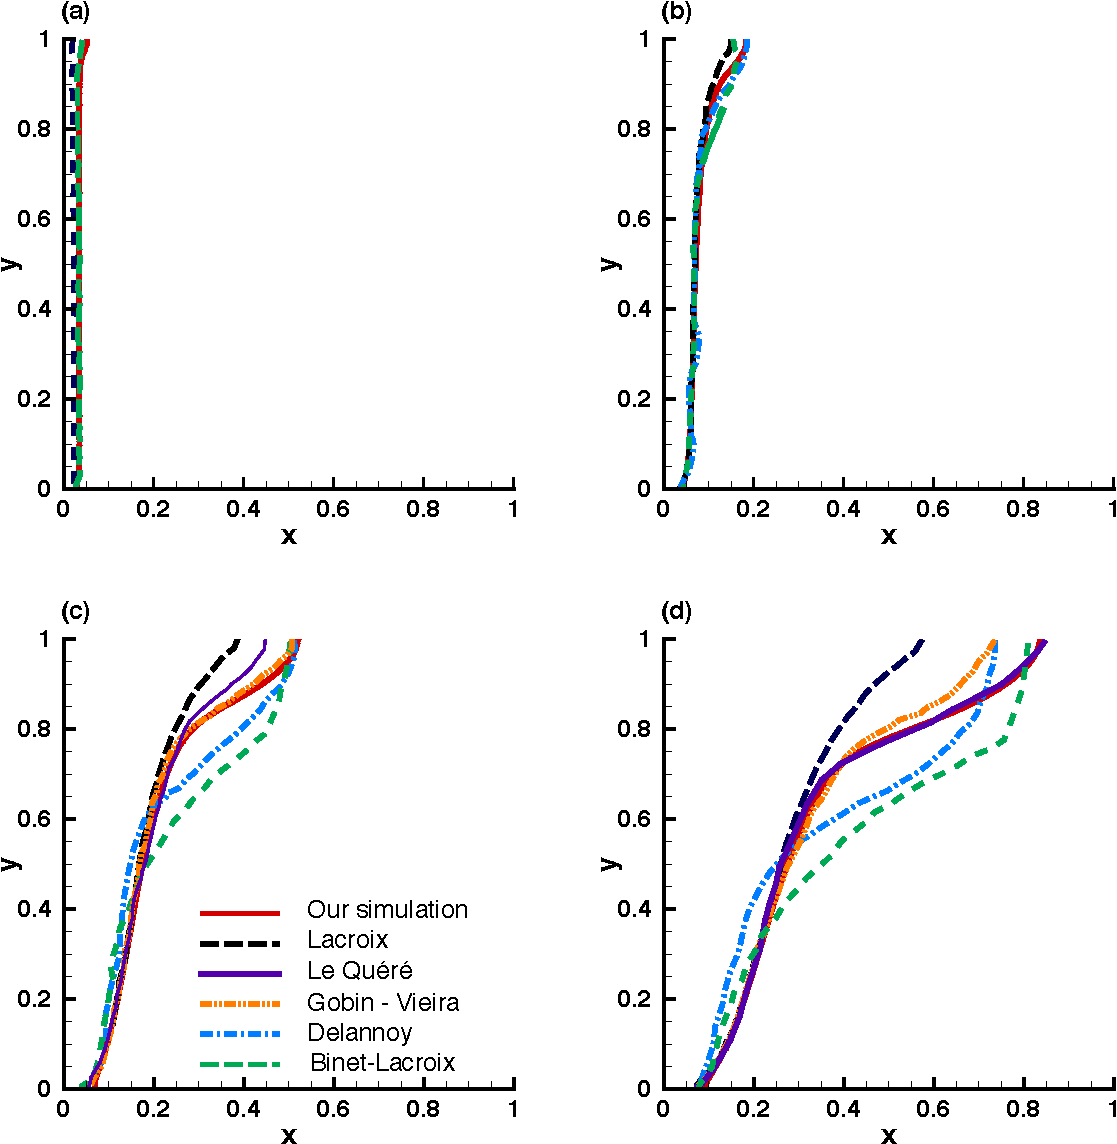
\includegraphics[width=\textwidth]{\figpath/Fig_cap_melting/fig03}
		\end{minipage}
	\end{center}
	\caption{Melting of a PCM (Benchmark 3). Location of the solid-liquid interface at dimensionless time (panels a to d) $\tau = 0.0005$,  $\tau = 0.002$, $\tau = 0.006$ and $\tau = 0.01$, compared with five simulations presented by \cite{bertrand1999melting}. 
	$\Ray = 2 \cdot 10^8$, $\Pr = 50$ and $\Ste = 0.1$.} \label{fig Bertran}
\end{figure}
\begin{figure}
	\begin{center}
		\begin{minipage}[t]{0.75\textwidth}
			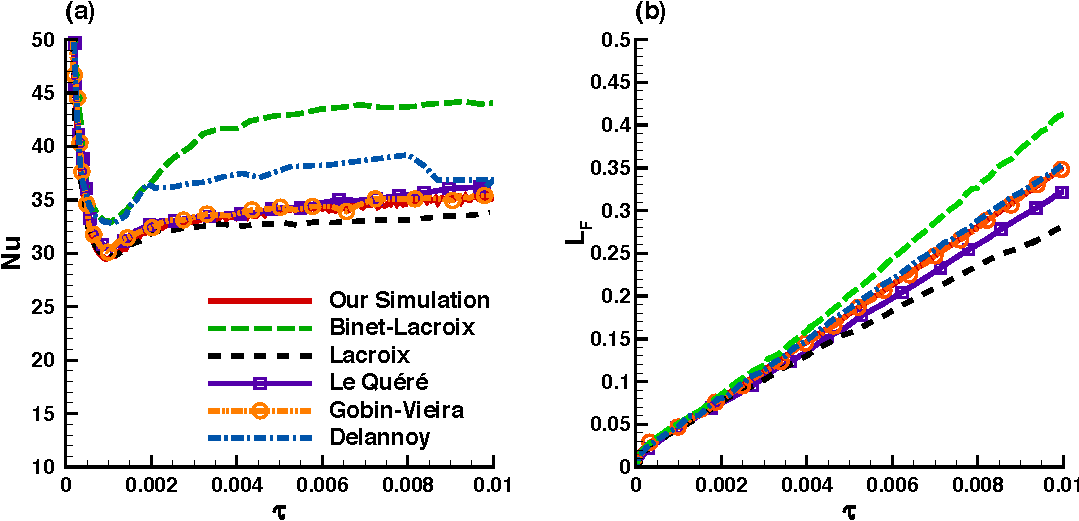
\includegraphics[width=\textwidth]{\figpath/Fig_cap_melting/fig04}
		\end{minipage}
	\end{center}
	\caption{Time evolution of the Nusselt number (a) and the liquid fraction (b) compared with five simulations presented by \cite{bertrand1999melting}.
	$\Ray = 2 \cdot 10^8$, $\Pr = 50$ and $\Ste = 0.1$.} \label{fig-Nu-Lf-Bertran}
\end{figure}
The phase-change interface for four time steps, $\tau = 5 \cdot 10^{-4}$, $\tau = 2 \cdot 10^{-3}$, $\tau = 6 \cdot 10^{-3}$ and $\tau = 1 \cdot 10^{-2}$ is represented in Figure \ref{fig Bertran}.
Our results are for each case in fairly good agreement with those of Gobin and those of  Le Qu{\'e}r{\'e}.
Gobin uses a front-tracking method using a coordinate transformation with a finite volume method with a $62 \times 42$ grids.
Le Qu�r� solves a single domain model using a second order scheme with a finite volume method with a $192 \times 192$ grids  (\cite{gobin2000melting}).\\
The time evolution of the Nusselt number and the liquid fraction are presented in Figure \ref{fig-Nu-Lf-Bertran}.
A very good agreement is obtained with Gobin and Le Qu{\'e}r{\'e}.
A relative difference, less than $2\%$ is noticed for the Nusselt number, and a dispersion, smaller than $4 \%$, for the melted fraction.\\
The high value of the Rayleigh number $\Ray = 10^8$ results in a very demanding numerical test.
The high velocity, inducing a very narrow thermal boundary layer can lead to unrealistic results and some numerical methods have failed.
The interest of the mesh adaptation is clearly evidenced since we  initially use only $40 \times 40$ grid points.



\subsection{Analysis of the time evolution of the melting process} \label{sec-melting}

We now pay a closer attention to the temporal evolution of different physical parameter of the system, during the melting phase.
We consider the following physical parameters:
$\Ray = 3.27 \cdot 10^5$, $\Pr = 56.2$ and $\Ste = 0.045$.

%\subsubsection{Time evolution} 

We start by analysing the time evolution of the melting process. At $\tau=0$, the material is solid and the initial temperature is set to $\theta_0=-0.01$ everywhere inside the cavity. Then, the temperature of the left wall is suddenly increased to $\theta_h=1$, while the right wall is maintained at the same cold temperature $\theta_c=-0.01$. The material starts to melt, with a melting (identified by the iso-line $\theta=\theta_f=0$) propagating from the left to the right side of the domain. The time evolution of the phase-change system is depicted in Fig. \ref{fig:melt-field} for representative time instants, also reported in previous studies.
\begin{figure}
	\begin{center}
		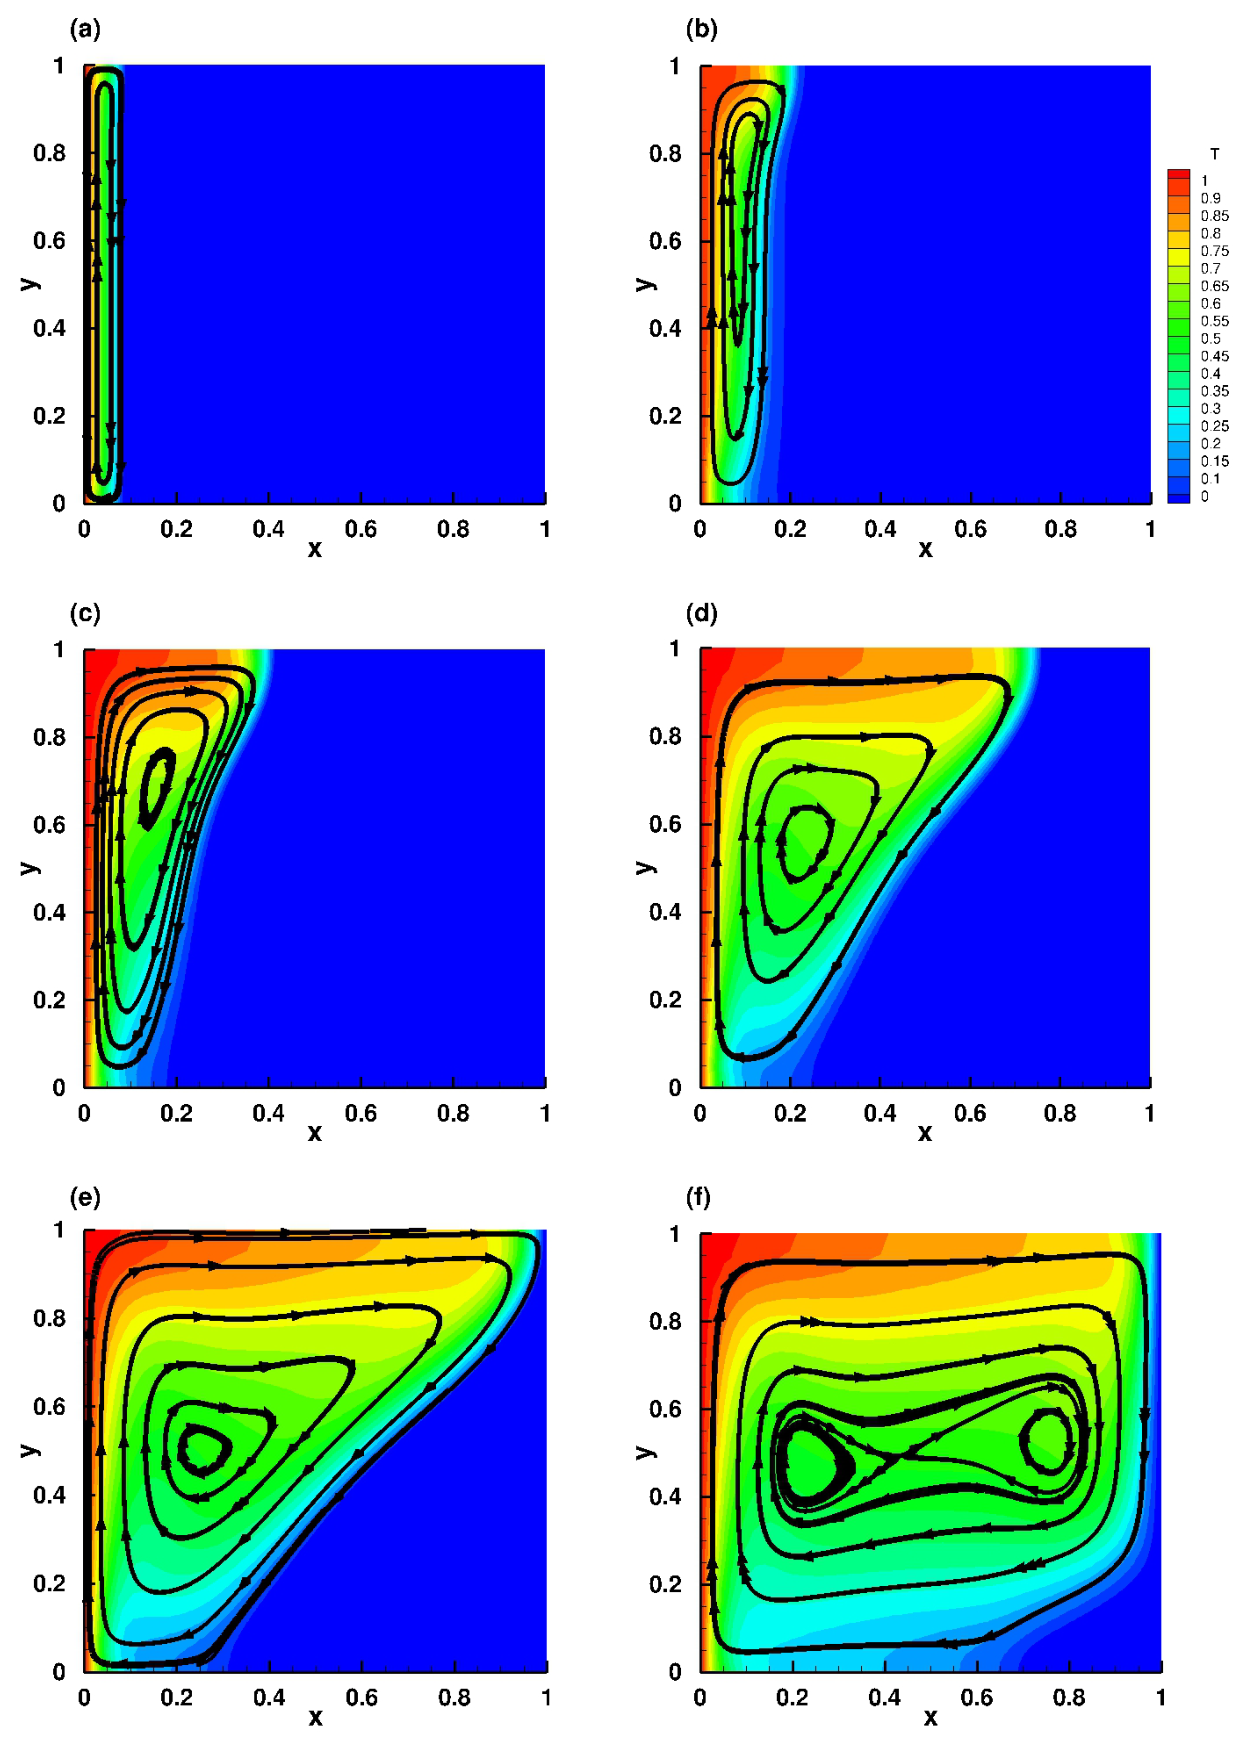
\includegraphics[width=.9\textwidth]{\figpath/Fig_cap_melting/fig05}
	\end{center}
	\caption{Complete melting of the PCM. Temperature iso-lines and streamlines in the fluid phase. The solid part is represented in blue and corresponds to the region of temperature $\theta \leq \theta_f=0$. Time instants (panels  a to f): $\tau=0.004; 0.016; 0.032; 0.063; 0.08; 0.2$. $\Ray = 3.27 \cdot 10^5$, $\Pr = 56.2$ and $\Ste = 0.045$.
		}\label{fig:melt-field}
\end{figure}


From Fig.  \ref{fig:melt-field}, we can easily identify three different regimes describing the time evolution of the melting process. 
\begin{itemize}
	\item From $\tau=0$ to $\tau =0.004$ (Fig.  \ref{fig:melt-field}a), we note the vertical shape of the melting front, well predicted by the classical conduction model of \cite{stefan1891theorie}. This indicates that, at this stage, heat transfer is dominated solely by conduction.
	
	 \item Between $\tau =0.016$ to $\tau =0.032$ (Fig.  \ref{fig:melt-field}b), the natural convection in the fluid phase starts to alter the shape of the melting front.
	A mixed conduction and convection regimes rule the heat transfer. 	Convection mainly affects the upper part of the fluid motion, while conduction is still dominating in the lower part. As the volume thermal expansion coefficient $\beta$ is positive, we expect a clockwise circulation of the liquid inside the convection cell, as noted by \cite{jany1988scaling}.
	This also makes the liquid-solid interface to move faster at the top of the cavity, explaining the deformed shape of the melting front, which is a signature of the convection effects  (see also \cite{kowalewski2004phase}). 
	
	\item After $\tau=0.032$ (Fig.  \ref{fig:melt-field}c-d), natural convection dominates the heat transfer process and impacts radically the solid-liquid interface shape and motion.
	The melting front line exhibits four distinct regions characterized by different slopes with respect to the vertical axis. The largest slope is observed at the top of the cavity and is related to the particular shape of the convection cell. Note that top and bottom parts of the interface are normal to the cavity boundaries because of the imposed adiabatic boundary conditions.

	\item After $\tau =0.08$  the melting front is nearly touching the right wall of the cavity, firstly at the top (Fig.  \ref{fig:melt-field}e) of the cavity. The melting process continues and the fluid progressively fills the cavity, with a melting front  deforming to a vertical line. The  simulation of the melting process is stopped at $\tau =0.2$ (Fig.  \ref{fig:melt-field}f), when it is numerically difficult to separate the melting front from the right wall boundary. At this time instant,  the fluid fraction reaches the value of $0.95$ and  the melting of the PCM is considered to be complete, even though a small region of solid PCM remains at the lower right bottom of the cavity. Note from Fig.  \ref{fig:melt-field}f the existence in the fluid  of two recirculating zones instead of a single one observed during previous stages.
	
\end{itemize}

\subsection{Scaling analysis} \label{sec:scaling anal}

The melting of the octadecane was theoretically studied by  \cite{jany1988scaling}. Combining scaling theory and numerical modelling, they suggested closed-form correlations for the temporal evolution of the average Nusselt number $N\!u$ defined at the hot boundary ($x=0$), under the form:
\begin{equation} \label{eq-Nu-scale}
N\!u(\tau) =  \frac{1}{\sqrt{2 \tau}} + \left[c_1 \Ray^{1/4} - \frac{1}{\sqrt{2 \tau}} \right]  \left[ 1 + \left(c_2 \Ray^{3/4}  \tau^{3/2}\right)^n \right]^{1/n}.
\end{equation}
The values of the constants were fitted from numerical data: $c_1 = 0.27$, $c_2 = 0.0275$, and $n=-2$. 

In Fig. \ref{fig:Nusselt} we compare the time evolution of the Nusselt number obtained from our numerical data (see Figure \ref{fig: pcm-case})  to experimental results of  \cite{Okada1984}  and predictions obtained from the correlation (\ref{eq-Nu-scale}). Our results perfectly fit the theoretical prediction of \cite{jany1988scaling}. They are also in good agreement with experimental data, suggesting, however, that very accurate measurements and numerical simulations are needed to validate theoretical scaling analysis.

The time evolution of the Nusselt number can be correlated with the different heat transfer regimes analysed in the previous section: 
\begin{enumerate}
	\item A pure conduction regime for $\tau  \gtrsim 0$  (corresponding to Fig.  \ref{fig:melt-field}a), characterized by the law $N\!u \sim (2 \tau)^{-1/2}$.
	Since the temperature gradient has initially huge values because of the sudden increase of the temperature of the left wall, the Nusselt number rapidly decreases during the first stage of the flow evolution. The evolution law $N\!u \sim \tau^{-1/2}$ can be also obtained from the Neumann exact solution of \cite{grigull1984heat}. 
	The  signature of this conduction regime is the slow heat transfer characterized by a monotonic decrease of the Nusselt number, down to a minimum value obtained for  $\tau \sim \Ray^{-1/2} =0.02$.
	
	\item A mixed conduction-convection regime  for $  0.02  \leq \tau \leq 0.05$ (illustrated in  Fig.  \ref{fig:melt-field}b). The influence of the Rayleigh number in  (\ref{eq-Nu-scale}) starts to be important and a good approximation for this regime is: $ N\!u \sim \tau^{-1/2} + \Ray\, \tau^{3/2}$.
	

	\item A convection dominated regime for $\tau > Ra^{-1/2}$  (corresponding to Figs.  \ref{fig:melt-field}c-e). In the asymptotic limit of large $\tau$, the simplified law $ N\!u \sim \Ray^{1/4}$ is obtained.
	The plateau at the value of $\Ray^{1/4}$ corresponds to the pure convective transfer and is observed in Fig. \ref{fig:Nusselt} for $  0.05 \leq \tau \leq 0.1$. Numerical results show a slight decrease of the $N\!u$ in the final stage ($\tau \geq 0.1$), when the melting front starts to touch the right wall of the cavity (see Figs.  \ref{fig:melt-field}e-f). The correlation model of \cite{jany1988scaling} is not valid for this late evolution of the melting process.
\end{enumerate}

\begin{figure}
	\begin{center}
		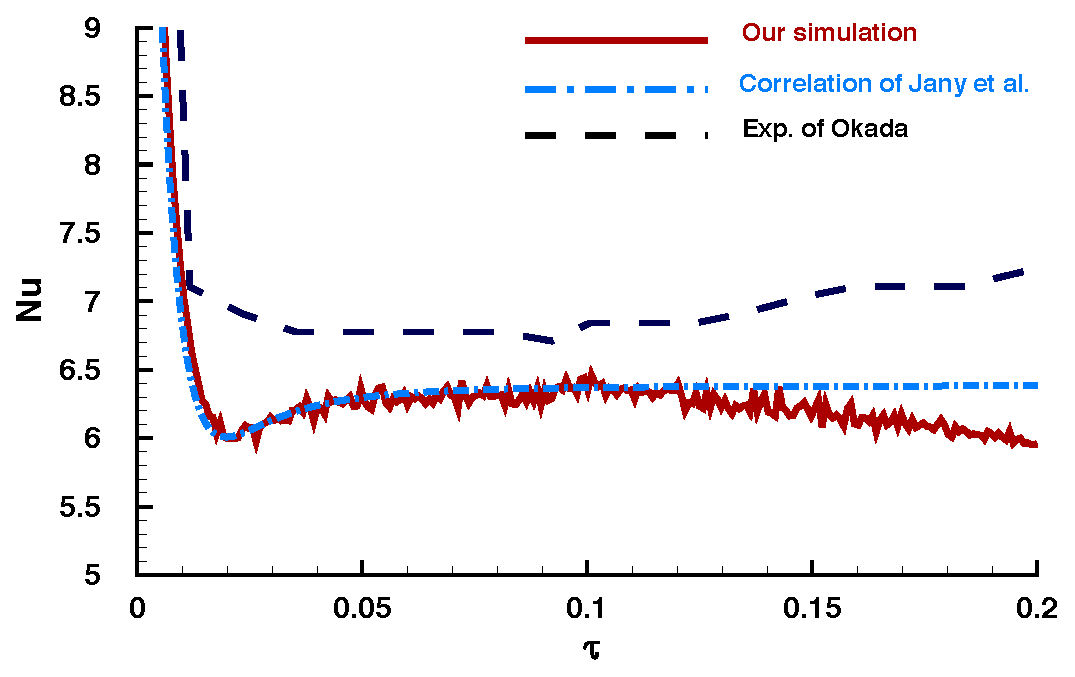
\includegraphics[width=0.7\textwidth]{\figpath/Fig_cap_melting/fig06}
	\end{center}
	\caption{Complete melting of the PCM. Time evolution of the average Nusselt number defined at the hot (left) wall (cf. eq. \ref{eq-Nu}) (solid line). Comparison with the experimental results of  \cite{Okada1984} (dashed line) and the predictions using the correlation (\ref{eq-Nu-scale}) suggested by \cite{jany1988scaling} (dash-dot line). $\Ray = 3.27 \cdot 10^5$, $\Pr = 56.2$ and $\Ste = 0.045$.}\label{fig:Nusselt}
\end{figure}


Another important basic quantity describing the melting process is the liquid fraction $L_f$.  
The time evolution of the liquid fraction (Fig. \ref{fig:Lf}a) displays three regimes during the melting process. $L_f$  initially grows as $\tau^{ 1/2}$, which is a typical law for a conduction-dominated heat transfer. Then, a linear temporal evolution is observed, until the melting front reaches the right wall.
This linear regime corresponds to the quasi-steady state observed in the evolution of the Nusselt number (Fig. \ref{fig:Nusselt}).

Using the asymptotic limits of Eq. (\ref{eq-Nu-scale}) for $ \tau \to 0$ (pure conduction) and $ \tau \to \infty$ (pure convection),  \cite{jany1988scaling} suggested the following correlation law for the time evolution of the liquid fraction:
\begin{equation} \label{eq-Lf-scale}
L_f(\tau) = \left[\left({\sqrt{2 \tau}} \right)^5 + \left(c_1 \Ray^{1/4}  \tau \right)^{5} \right]^{1/5},
\end{equation}
where $c_1=0.27$ is the same constant as in (\ref{eq-Nu-scale}). We compare in Fig. \ref{fig:Lf}b our numerical results with the predictions based on (\ref{eq-Lf-scale}) within the validity domain of the analysis, \ie before the melting front reaches the right wall of the cavity. A very good agreement is found with theoretical predictions and also with previously published numerical results \citep{Wang2010}.

\begin{figure}[!h]
	\begin{center}
		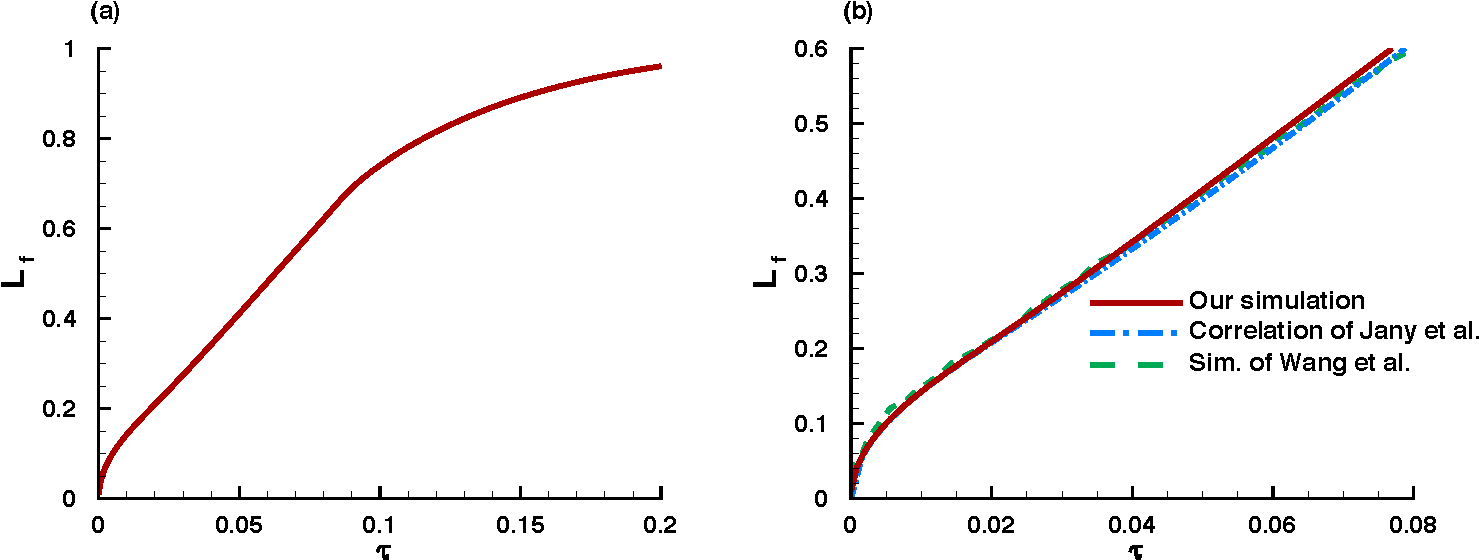
\includegraphics[width=0.9\textwidth]{\figpath/Fig_cap_melting/fig07}
	\end{center}
	\caption{Complete melting of the PCM. (a) Time evolution of the liquid fraction for the complete melting of the PCM. (b) Comparison of our results (solid line) with the numerical results of  \cite{Wang2010} (dashed line) and the predictions using the correlation (\ref{eq-Lf-scale}) suggested by \cite{jany1988scaling} (dash-dot line).}\label{fig:Lf}
\end{figure}




%%%%%%%%%%%%%%%%%%%%%ù
\subsection{Influence of the Rayleigh number}
%%%%%%%%%%%%%%%%%%%%%

To assess the influence of the Rayleigh number on the evolution of the melting process, we performed two other simulations by multiplying the initial value of $\Ray = 3.27 \cdot 10^5$ by a factor of 5 and 10, respectively. The exact values are: $\Ray = 1.62 \cdot 10^6$ and $\Ray = 3.27 \cdot 10^6$. 
First, we increase the height $H$ of the cavity by a factor of $\sqrt[3]{5}$ and $\sqrt[3]{10}$ and consider the same $\delta T$.
Thus the Stefan number $\Ste$ is kept constant.
Second, we increase the temperature difference parameter $\delta T$ by keeping $H$ constant.
It corresponds of an increased value of the Stefan number by a factor of $5 $ and $10$:
$\Ste = 0.223$ and $\Ste = 0.45$.
Figures \ref{fig:Ra-Nusselt-H} and \ref{fig:Ra-Nusselt-deltaT} show the temporal evolution of the liquid fraction $L_f$ (a),  and the average Nusselt number defined at the hot wall,  (b). 
The same heat transfer regimes described previously are observed for each case: conduction, mixed conduction-convection and convection.

Figure \ref{fig:Ra-Nusselt-H}(a) indicates that increasing the Rayleigh number by keeping $\delta T$ constant induces a slower melting rate.
This is the expected behaviour since the size of the PCM is increased by a factor of 2, and the velocity $\vec u$ is hence decreasing  in order to satisfy the condition $\Rey = 1$.
We note however a non-monotonic variation of time necessary to melt a fixed value of fluid.
For instance, to achieve $L_f = 0.5$ (50\% of the volume is melted), an increase of $\Ray$ by a factor of $10$ leads to a growth of the time by a factor of $1.7$.
Nonetheless, when $\Ray$ is  $5$ times larger, the necessary time only increases by a factory of $2$.
This is most likely due to the non-linear intricacies of the problem and requires further investigation.
Furthermore, the Nusselt number reported in Figure \ref{fig:Ra-Nusselt-H}(b) shows that the higher the Rayleigh number, the higher the Nusselt number.
This is consistent, since the temperature gradient is integrated along a greater heated wall. 

Figure \ref{fig:Ra-Nusselt-deltaT}(a) shows that by increasing the value of $\delta T$ and consequently increasing the Rayleigh number and the Stefan number, the PCM melts faster. 
We note that the heigh $H$ of the cavity is kept constant, hence the natural convection flow in the melted PCM is enhanced when the Rayleigh number keep increasing.
As a consequence, the convection-dominated regime is reached earlier, as shown by the shift of the minimum of the $N\!u$ to lower values of $t_{\varphi}$ in Figure \ref{fig:Ra-Nusselt-deltaT}(b). This evolution is also observed for the liquid fraction. 
As expected, an increase of the Rayleigh number and the Stefan number is followed by an enhancement of the heat transfer during the melting, and consequently an improved efficiency of the PCM.
\begin{figure}
	\begin{center}
		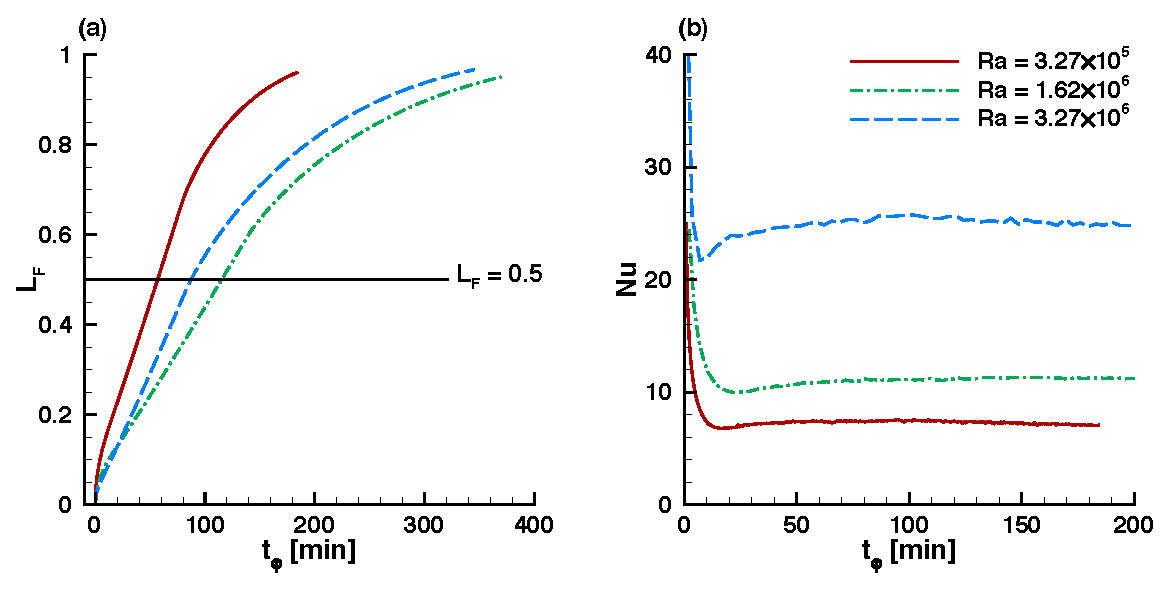
\includegraphics[width=0.95\textwidth]{\figpath/Fig_cap_melting/fig08}
	\end{center}
	\caption{Complete melting of the PCM.  Influence of the value of the Rayleigh number ($\Ray$) on the time evolution of the average Nusselt number defined at the hot (left) wall (a) and liquid fraction (b). The reference case ($\Ray=3.27\cdot 10^5$) is represented by red continuous lines. The value of the $\Ray$ was increased by a factor of $5$ and $10$, respectively while the Stefan number $\Ste$ is kept constant.}\label{fig:Ra-Nusselt-H}
\end{figure}

\begin{figure}
	\begin{center}
		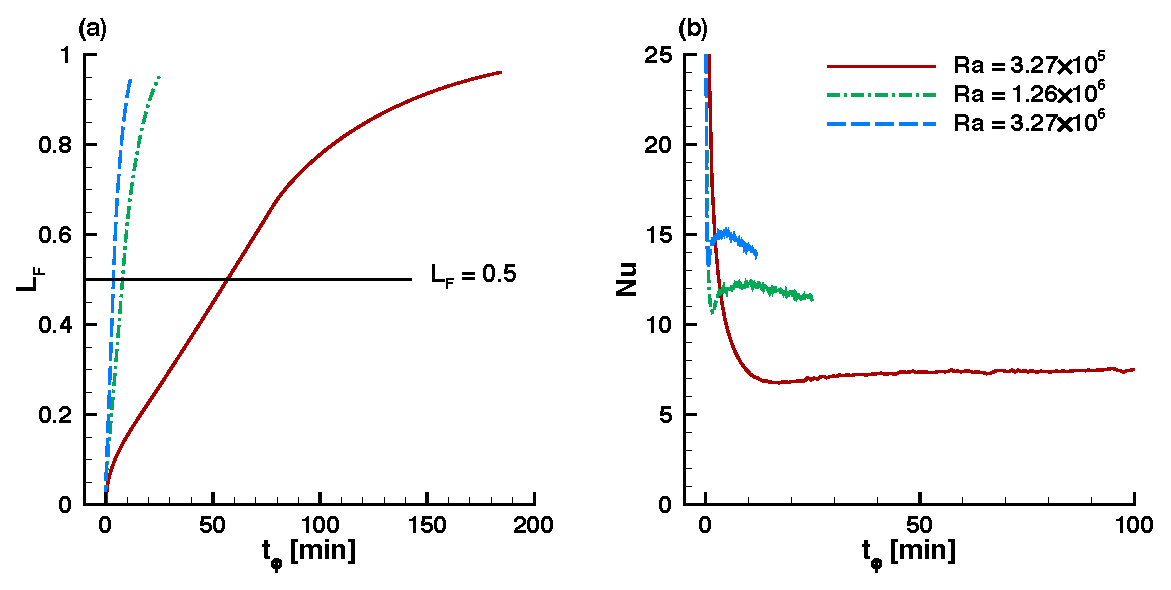
\includegraphics[width=0.95\textwidth]{\figpath/Fig_cap_melting/fig09}
	\end{center}
	\caption{Complete melting of the PCM.  Influence of the value of the Rayleigh number ($\Ray$) on the time evolution of the average Nusselt number defined at the hot (left) wall (a) and liquid fraction (b). The reference case ($\Ray=3.27\cdot 10^5$) is represented by red continuous lines. The value of the $\Ray$ and $\Ste$ were increased by a factor of $5$ and $10$, respectively.}\label{fig:Ra-Nusselt-deltaT}
\end{figure}


%After the validation of the Navier-Stokes-Boussinesq solver, we test in this subsection the numerical system solving the model (\ref{eq-newton-C1}) for  a phase-change system with convection. 
%Two new non-linearities are considered in the system: the Carman-Kozeny penalty term and the enthalpy source term $S$. 
%$S$ is regularized using the same function (\ref{eq-Stanh}), with $S_s=0$, $S_l=1/\Ste$, where $\Ste$ denotes the Stefan number. 
%Five cases are computed and detailed in Table \ref{tab-melt-cases}.
%\begin{itemize}
%\item Case $\#1$ reproduces the experimental study of \cite{Okada1984}, it consists of a differentially heated square cavity, filled with octadecane paraffin.
%\item Case $\#2$ reproduces the simulation of \cite{bertrand1999melting}. The accuracy of different numerical methods were compared in the paper of \cite{bertrand1999melting} and allows us thus to compare our numerical method with existant code.
%\item Case $\#3$ reproduces the melting of a cylindrical PCM with heated inner tube. The results are compared with the numerical data of \cite{luo2015lattice}.
%\item Case $\#4$ reproduces the melting of Gallium in a rectangular cavity heated by the sidewall, simulated by \cite{hannoun2003resolving}.
%\item Case $\#5$ reproduces the simulation of \cite{nourgaliev2016fully} using highly distorted mesh to simulate a natural convection with solid crush formation.
%\end{itemize}

%The authors cited before have used different dimensionless times for each simulation cases. 
%\cite{luo2015lattice} used the Fourier dimensionless time $Fo$ for example, while \cite{bertrand1999melting} used dimensionless time $\tau$, defined as follows:
%
%\begin{equation}
%\label{eq-adim-tau}
%\tau = Ste\cdot Fo = Ste\cdot \frac{\alpha t_{\varphi}}{H^2}  = Ste\cdot \frac{t}{Pr},
%\end{equation}
%with $t_{\varphi}$ the physical time and $t$ the non-dimensional time defined in (\ref{eq-adim}).
%So, our result will be presented using different dimensionless time depending on each cases.
%Details are reported on Table \ref{tab-melt-cases}.
%\begin{table}
%\centering
%\begin{tabular}{*{6}{c}}
%   & case $\#1$ & case $\#2$ & case $\#3$ & case $\#4$ &case $\#5$ \\
%  \toprule 
% $Ra$ & $3.27 \cdot 10^5$ & $10^8$ & $5 \cdot 10^4$ & $7 \cdot 10^5$ & $10^6 $\\
% $Pr$ & $56.2$ & $50$ & $0.2$ & $0.0216$ & $0.1$ \\
% $Ste$ & $0.045$ & $0.1$ & $0.2$ & $0.046$ & $4.854$ \\
% \midrule
% $\delta t$ & $0.1$ & $10^{-3}$ & $10^{-4}$ & $10^{-4}$ & $10^{-2}$ \\
% Triangle & $5,200$ & $20,000$ & $5,300$ & $7,500$ & $11 ,000$ \\
% dimensionless t & $t$ & $\tau$ & $Fo$ & $t_{phys}[s]$ & $t$ \\
% $V_{ref}$ &  $\frac{\nu_l}{H}$ & $\frac{\nu_l}{H}$ & $\frac{\nu_l}{H}$ & $\frac{\nu_l}{H}$ & $\frac{\nu_l}{H} \sqrt{\frac{Ra}{Pr}}$ \\
%  \bottomrule
% \end{tabular}
%\caption{Parameters for the melting cases.}
%\label{tab-melt-cases}
%\end{table}

%\subsubsection{Melting of an octadecane PCM in a square cavity} \label{sec-case1}
%First, the melting of an octadecane PCM in a square cavity of height $H=1.5$ cm is of interest. 
%For this case both experimental and numerical results are available \citep{dan-2014-JCP,Okada1984,Wang2010,Ma2006}. 
%The material characteristics (specific heat $C$ and conductivity $K$) are considered constant, as in previous numerical studies of \cite{Wang2010,Ma2006}. 
%The material is initially solid ($\theta_0=-0.01$) and melts progressively starting from the left boundary, maintained at hot dimensionless temperature $\theta_h=1$.  
%The right boundary is also isothermal with cold temperature $\theta_c=-0.01$, and the horizontal boundaries are adiabatic.
%
%The computation starts from a refined mesh near the hot boundary and then uses mesh adaptivity at each time step. 
%{The mesh is refined using metrics computed from three variables: the two fluid velocities and the  enthalpy source term $S$. 
%To reduce the impact of the interpolation on the global accuracy, we use two successive fields $(S^n)$ and $(S^{n+1})$ in the adaptivity procedure.} This allows to well refine the fluid part of the domain and the artificial mushy region around the interface. A picture of the mesh at dimensionless time $t=78.7$ is presented in Figure \ref{fig:pcm-valid}a. 
%
%We compare the position of the phase-change interface at $t = 39.9$ and $t=78.7$ with the experimental data by \cite{Okada1984} and previously published numerical results by \citep{Wang2010,dan-2014-JCP} in Figure \ref{fig:pcm-valid}b. 
%The obtained shape and position of the liquid-solid interface is closer to experimental results than numerical results reported in \cite{Wang2010}.
%This is a direct consequence of the mesh adaptivity capabilities of our method.
%
%This comparison also allowed us to finely tune the value of the constants used in the model (\ref{eq-CK}). 
%Even though it is generally assumed that a large value for $\CKC$ must be set, the exact value of this constant could influence the accuracy of the results \citep{kheirabadi2015effect, Kumar2017}. 
%This choice of the value of this constant is a still open problem.  
%Very good agreement with the experimental result of \cite{Okada1984} is obtained for $\CKC$ varying in the range $[10^6, 10^8]$. 
%Nevertheless, imposing  a too large value $\CKC=10^{10}$ results  in artificially slowing the propagation of the melting front. We set for all subsequent simulations $\CKC= 10^6$.
%
%Quantitative validation was performed for the melting of octadecan in this part, and the numerical assessment is in very good agreement with experimental  and other numerical results.
%
%\begin{figure}
%	\begin{center}
%		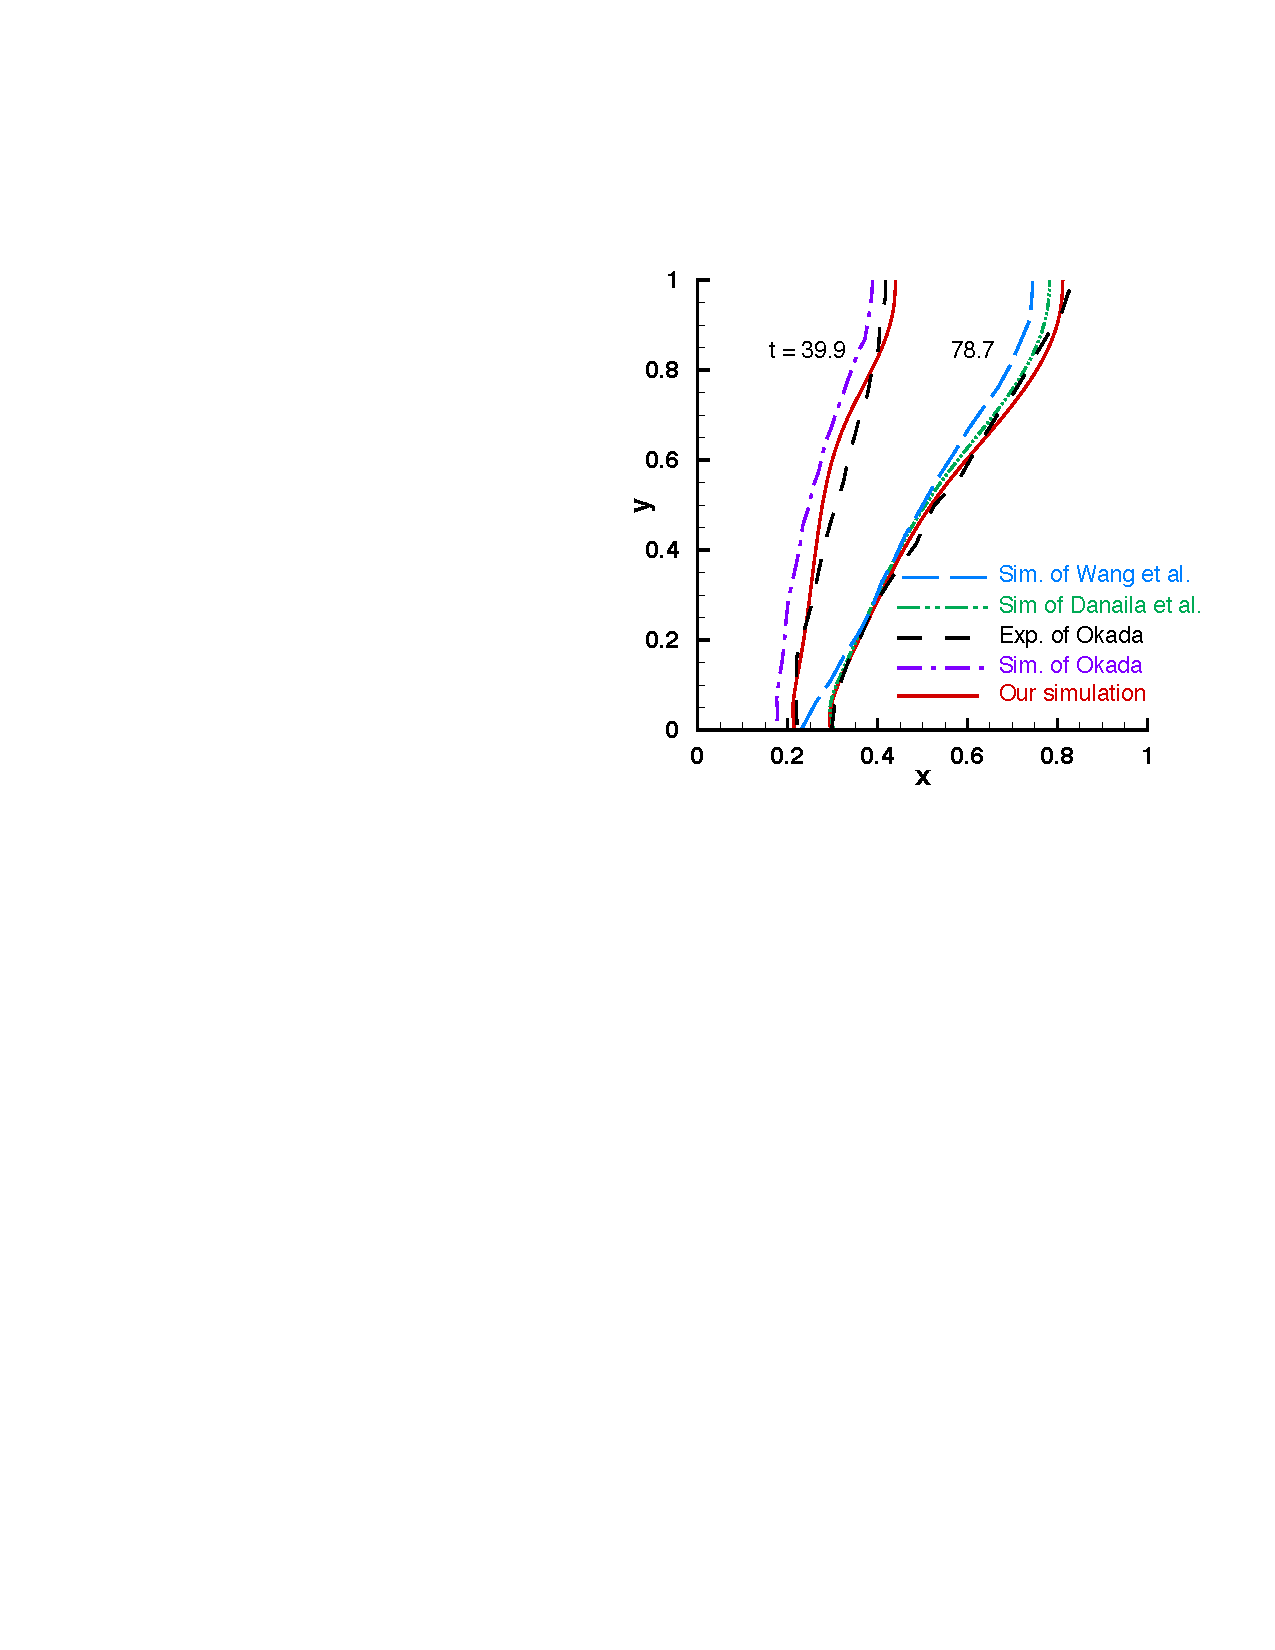
\includegraphics[width=0.9\textwidth]{\figpath/Fig_cap_melting/MELT_cavity_valid_2}
%	\end{center}
%	\caption{Case $\#1$ Melting of the PCM. (a) adapted finite-element mesh at time instant $t=78.7$.  (b) Comparison with experimental data of \cite{Okada1984} and numerical results of \cite{dan-2014-JCP} and \cite{Wang2010} for two time instants ($t=39.9$ and $78.7$).}
%	\label{fig:pcm-valid}
%\end{figure}
%
%\subsubsection{Melting of an octadecane PCM with high Rayleigh number}
%The domain of interest in this section is the same as presented in \ref{sec-case1} by increasing the Rayleigh number by a factor of $300$ (see Table \ref{tab-melt-cases}).
%This case is very challenging since the natural convection becomes important in the fluid flow, and enhances considerably the heat transfer.
%
%\cite{bertrand1999melting} compiled results provided by five different authors (Lacroix, Le Qu{\'e}r{\'e}, Gobin-Vieira, Delannoy and Binnet-Lacroix). Results provided by these investigators will be hereafter referred to as (say) 'Lacroix, from \cite{bertrand1999melting}'.
%They have attempted a first comparison by taking several numerical methods to compute the basic configuration presented in this section. 
%Two investigators among the five failed to predict the process and showed unrealistic behaviours in Figures \ref{fig Bertran}a and \ref{fig Bertran}b:
%Lacroix and Delannoy seem to be insufficiently converged as shown by Figure \ref{fig Bertran}a, and Binet-Lacroix overestimates the average Nusselt number by more than $30 \%$ (Figure \ref{fig Bertran}b).
%Hence, this collection of results allows us to compare our numerical method with the existant code and check if realistic results are obtained for complex physical configurations.\\
%We further inspect the melting front and the Nusselt number $N\!u$ at the left wall ($x=0$) for each of the five methods presented by \cite{bertrand1999melting}.
%The Nusselt number $N\!u$ is defined as follows:
%\begin{equation}\label{eq-Nu}
%N\!u = \int_{0}^1 \left(\frac{\partial \theta}{\partial x}\right)_{x=0}\, dy.
%\end{equation}
%
%\begin{figure}
%	\begin{center}
%		\begin{minipage}[t]{0.8\textwidth}
%			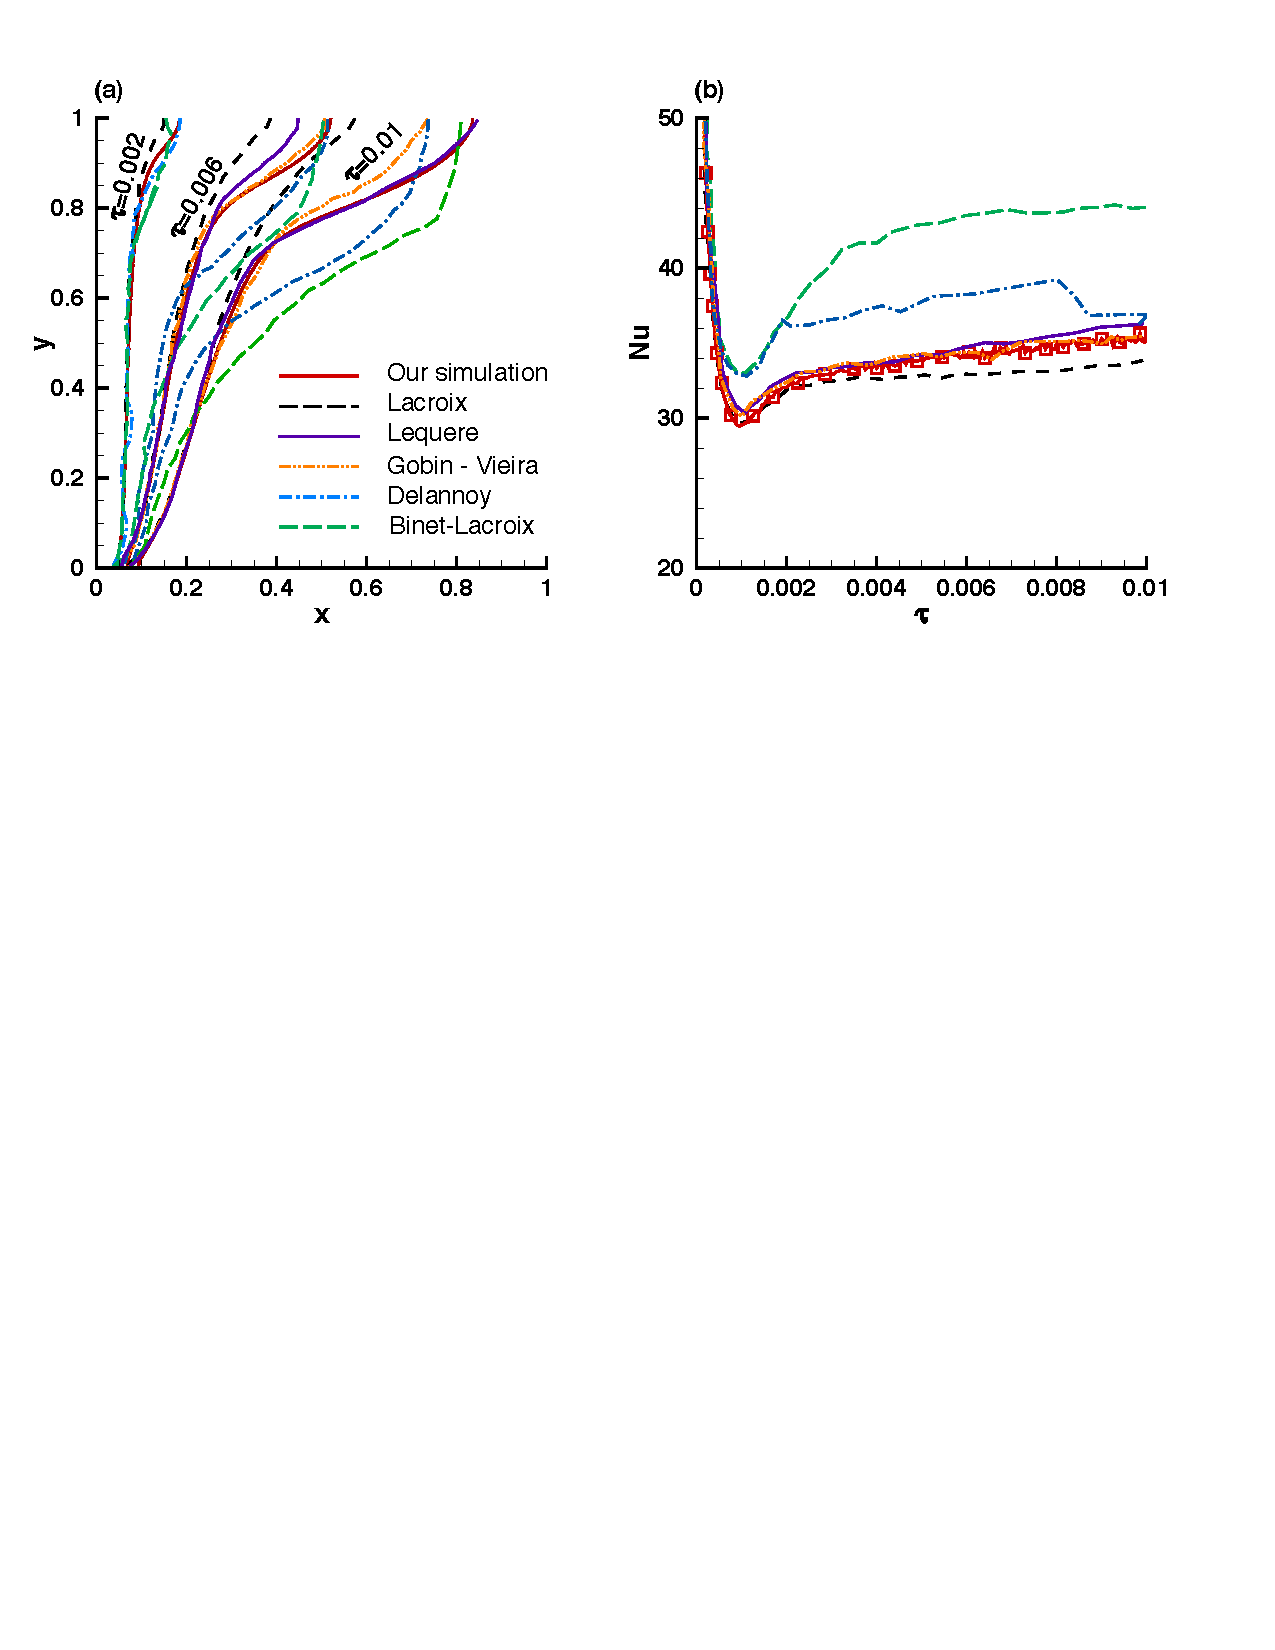
\includegraphics[width=\textwidth]{\figpath/Fig_cap_melting/Valid_Bertran}
%		\end{minipage}
%	\end{center}
%	\caption{Case $\#2$ Melting of the PCM with high Rayleigh number. Comparison with five investigators in \cite{bertrand1999melting}. (a) Location of the solid-liquid interfaces at dimensionless time $\tau = 0.002$, $\tau = 0.006$ and $\tau = 0.01$. (b) Temporal evolution of the Nusselt number.} \label{fig Bertran}
%\end{figure}
%
%The melting front for three time steps, $\tau = 2 \cdot 10^{-3}$, $\tau = 6 \cdot 10^{-3}$ and $\tau = 1 \cdot 10^{-2}$ is reported in Figure \ref{fig Bertran}a.
%Our results are for each case in fairly good agreement with those of Gobin and Le Qu{\'e}r{\'e}.  
%Details on the method and the numerical procedures are listed in \cite{gobin2000melting}.
%Gobin uses a front-tracking method using a coordinate transformation with a finite volume method in a $62 \times 42$ grid
%and Le Qu�r� solves a single domain method using a second order scheme with a finite volume method in a $192 \times 192$ grid. 
%The time evolution of the Nusselt number is presented in Figure \ref{fig Bertran}b.
%A very good agreement is still obtained with Gobin and Lequere.
%A relative difference, less than $2\%$ is noticed for the Nusselt number.
%
%The high Rayleigh number $Ra = 10^8$ is a very demanding numerical test.
%The high velocity, inducing a very narrow thermal boundary layer can lead to unrealistic result and some numerical method have failed.
%The interest of the mesh adaptation is clearly exhibited since we  initially use only $40 \times 40$ grid.

\section{Melting of PCM in complexe geometries: cylindrical evolving inclusions and distorted mesh}
\subsection{Melting of cylindrical PCM with inner heated tubes} \label{subsec-luo}

We have simulated previously, for both case $\#1$ and case $\#2$, phase change problems evolving in a square cavity.
A more complex geometry is studied in this section, by reproducing the configuration proposed by \cite{luo2015lattice}.
The interest is twofold: the geometry is challenging since is it complex and \cite{luo2015lattice} uses Lattice Boltzmann method, a microscopic model, which is different from previous validation cases.

Cylindrical PCM of dimensionless radius $R=1$ with tube inclusions are studied.
In fact, \cite{agyenim2010review} pointed out, in a critical review of materials used for heat storage, that more than $70\%$ of the PCM container are using the shell and the tube system.
We simulate three cases taking into account one heated tube, four heated tubes, and nine heated tubes with the same contact area.
For the one heated tube case, the radius $R_i$ of the inner tube is one-quarter of the outer tube ($R_i = R/4$), for four heated tubes $R_i = R/8$ and for nine heated tubes $R_i = R/12$.
A Dirichlet boundary condition is applied to inner tubes $\theta = \theta_h$,
and a Neumann boundary condition $\frac{\partial \theta}{\partial n} = 0 $ is used at the outers.
An homogenous Dirichlet boundary condition ($\vec u = 0$) is applied everywhere for the velocity.
Only the half of the domain is simulated since the problem is symmetric.
The mesh is refined initially around inner tubes, and is dynamically adapted at each time step around the melting front and the thermal boundary layer area.
The same metrics presented in \ref{sec-case1} are used for the mesh adaptation process.

The melting front (black line), the temporal evolution of the temperature field, and the time evolution of the liquid fraction, showing the effect of the configuration, are shown in Figures \ref{fig-Luo-Field} and \ref{fig-Lf-Luo}.
The configuration of the obstacles in the liquid phase, influences directly the fluid motion and the shape of melting front.
The more the number of inner tubes, the stronger the natural convection in the melted PCM.
Consequently the shape of the interface is impacted.
The heat transfer is hence enhanced, inducing a faster melting time: a ratio of $5.4$ is noticed from the melting time with nine and one tubes.

The evolution of the liquid fraction is compared with the numerical result of \cite{luo2015lattice} in Figure \ref{fig-Lf-Luo} and a good agreement is obtained.

\begin{figure}
	\begin{center}
		\begin{minipage}[t]{0.8\textwidth}
			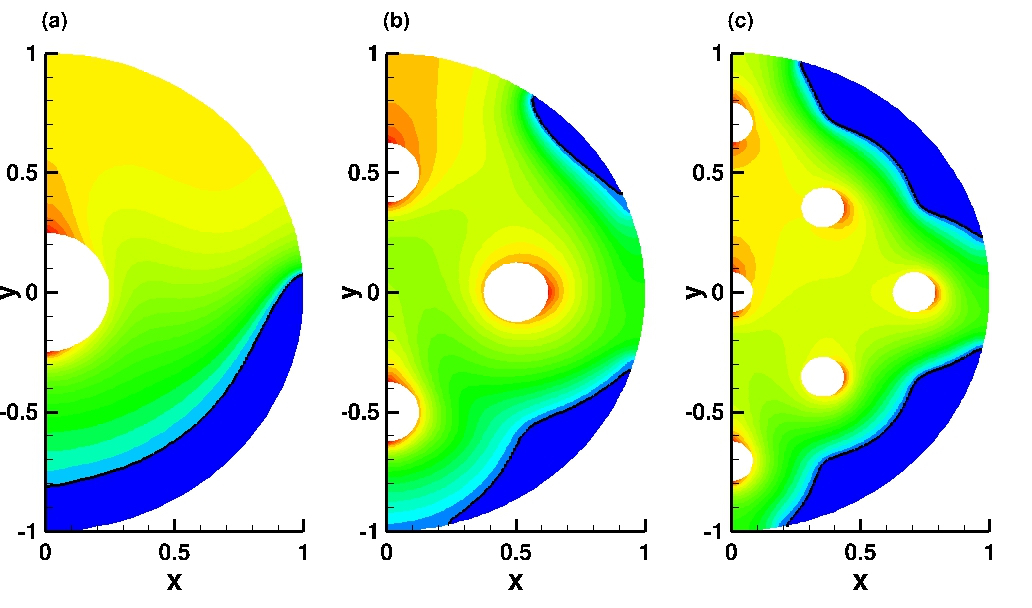
\includegraphics[width=\textwidth]{\figpath/Fig_cap_melting/MELT_Luo_Field}
		\end{minipage}
	\end{center}
	\caption{Case $\#3$ Temperature field for the melting of cylindrical PCM, in the half of the domain, with one (a), four (b), and nine (c) heated tubes.  
	$R_i = R/4$ for one heated tube, $R_i = R/8$ for four tubes and $R_i = R/12$ for nine tubes.
	Melting  front are localized with black lines.} \label{fig-Luo-Field}
\end{figure}

\begin{figure}
	\begin{center}
		\begin{minipage}[t]{0.5\textwidth}
			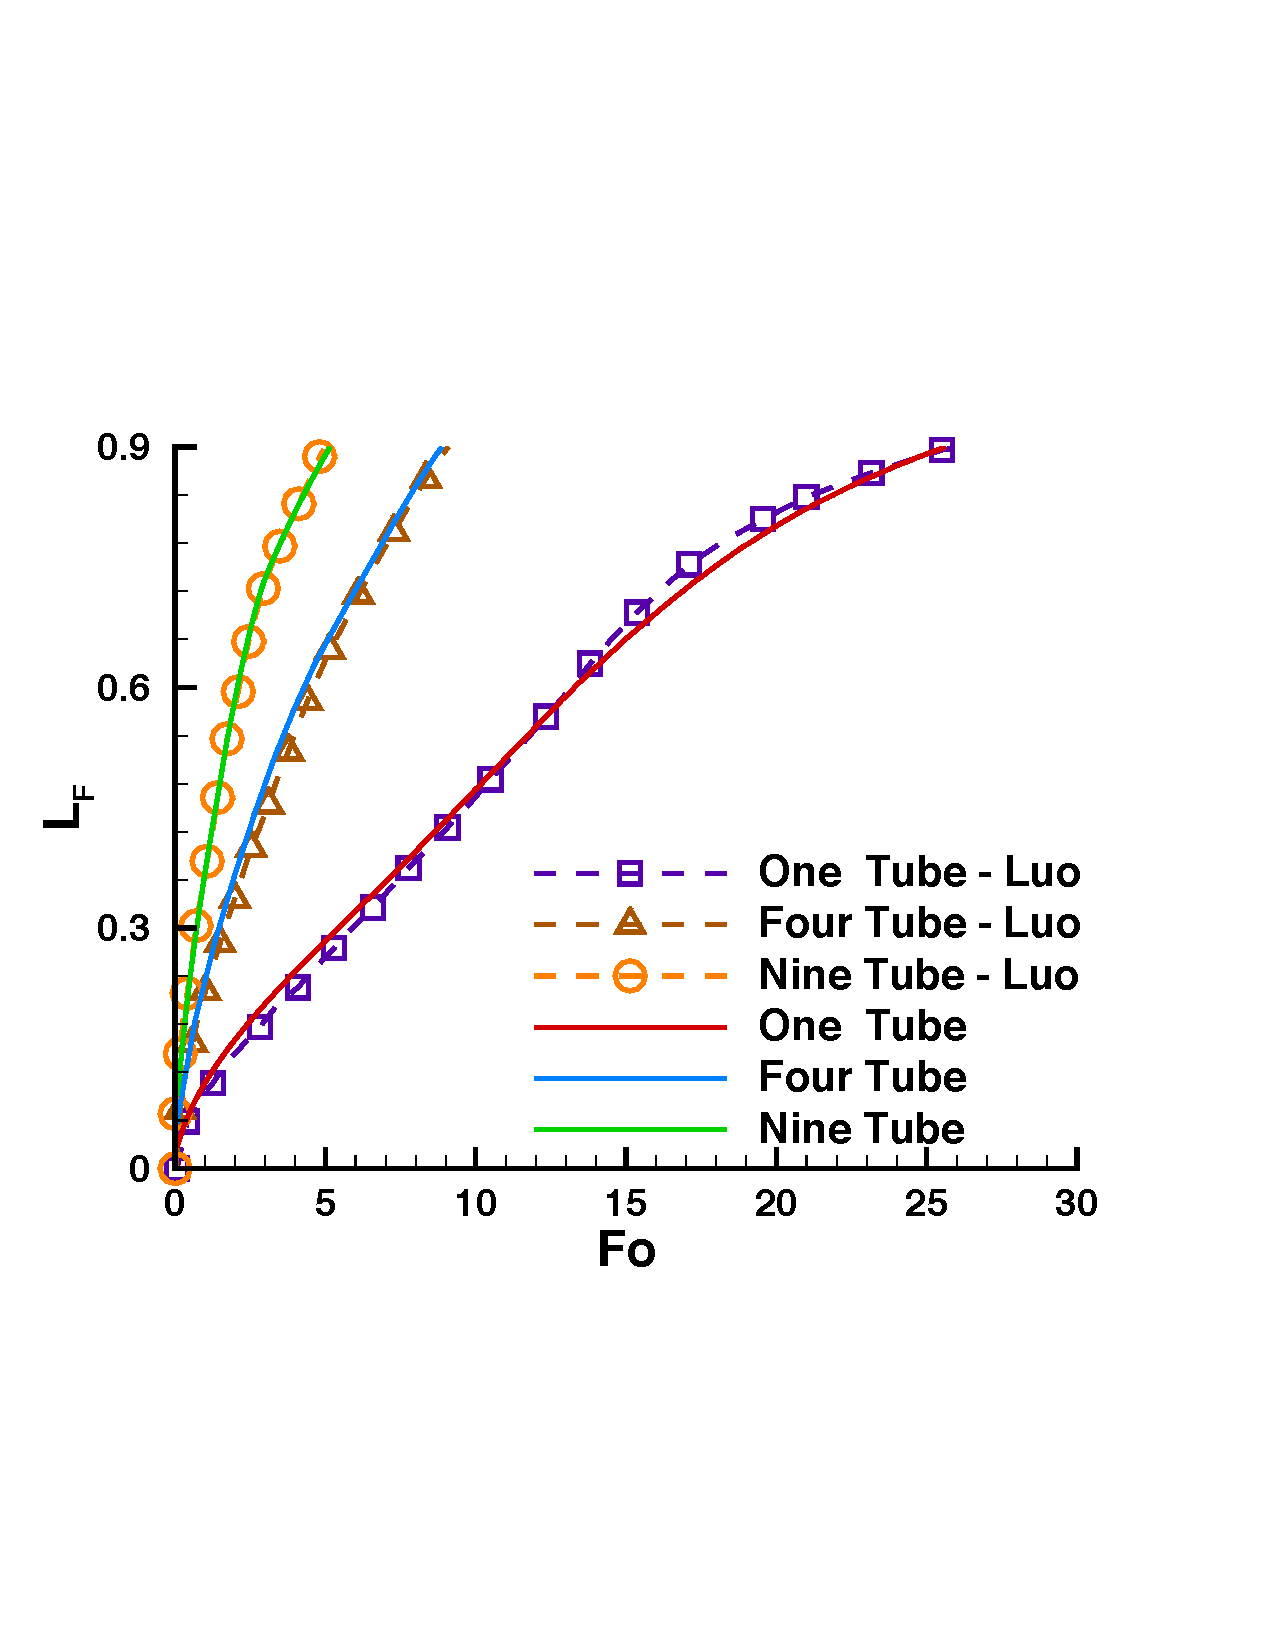
\includegraphics[width=\textwidth]{\figpath/Fig_cap_melting/Lf_Luo}
		\end{minipage}
	\end{center}
	\caption{Case $\#3$ Time evolution of the liquid fraction for one, four, and nine heated tubes. Comparison with numerical results of \cite{luo2015lattice}.} \label{fig-Lf-Luo}
\end{figure}

\subsection{Solid crust formation in a highly distorted mesh}

The solid crust formation inside a highly distorted domain, simulated by \cite{nourgaliev2016fully} is of interest in this section.
\cite{nourgaliev2016fully} used finite element with discontinuous Galerkin method.

The fluid is initially motionless with an initial dimensionless temperature $\theta_i = 2$.
The temperature of fusion is set to $\theta_f = 1.4$ according to \cite{nourgaliev2016fully} parameters.
It is worth noting that \cite{nourgaliev2016fully} have used $T_{ref} \ne T_f$ thus $\theta_f \ne 0$.

The left side is set at cold temperature $\theta_c = 1.39$ in the initial stage as the right wall was kept constant at a hot temperature $\theta_h = 2$, inducing a nearly steady-state natural circulation. 
The cold temperature at the left wall is then dropped down to $\theta_c = 1$, below the temperature of solidification starting the formation of a solid crust layer. 

\begin{figure}
	\begin{center}
		\begin{minipage}[t]{\textwidth}
			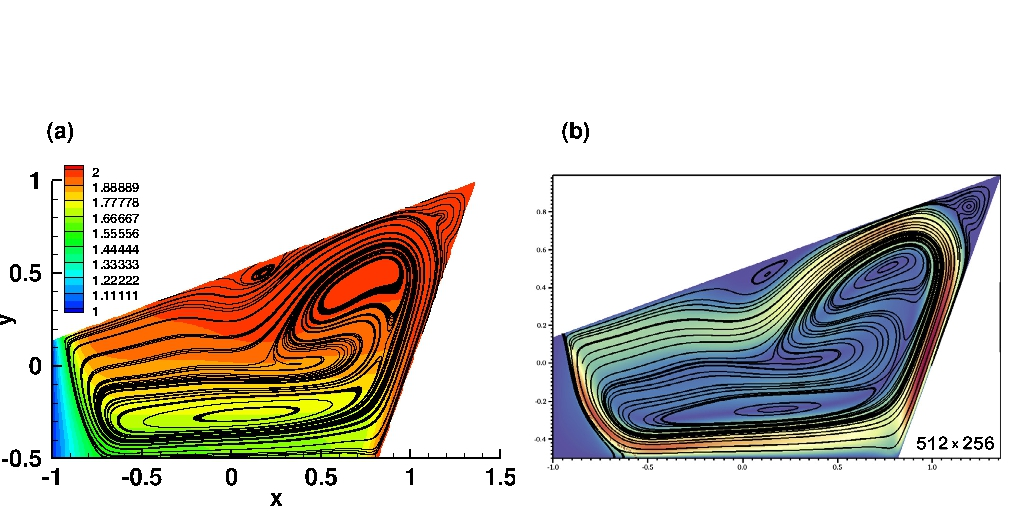
\includegraphics[width=\textwidth]{\figpath/Fig_cap_melting/Nourgaliev-Valid_2}
		\end{minipage}
	\end{center}
	\caption{Case $\#5$ Solid crust formation in a distorted mesh. Temperature field and streamlines of our simulation (a) and \cite{nourgaliev2016fully}  (b). } \label{fig-Nourgaliev}
\end{figure}

The temperature field and the streamlines are reported in Figure \ref{fig-Nourgaliev}.
We are qualitatively in a fairly good agreement with \cite{nourgaliev2016fully}.



\section{Melting of Gallium in a rectangular cavity}

The observation on the melting of the gallium in a rectangular cavity was a controversy since the question if  the flow in the fluid is monocellular of multicellular was raised by \cite{dantzig1989modelling}.
The experimental result exhibits indeed a monocellular structure, while many researchers claim this observation to be incorrect.
Prior to \cite{dantzig1989modelling} note, both experimental and numerical result support a single cell solution in the fluid phase.
Later, simulations provides solutions with multicellular flow. 
\cite{hannoun2003resolving} concluded that monocellular observation is caused by a problem of convergence of the numerical solution. It can be due to the grid size or inconsistencies in the mathematical model.

Therefore, this test case simulating the melting of the Gallium is a relevant exercice to test the consistency of our method.
To capture the very small cell during the first step of the melting, \cite{hannoun2003resolving} uses a $800 \times 1,120$ fixed grids in a rectangular domain of dimensions $6.35$ cm $\times \, 8.89$ cm. 
However, a maximum of $6 000$ triangles are necessary with our adaptive method to reproduce the numerical result of \cite{hannoun2003resolving}, that is a ratio of $10^2$.

\begin{figure}
	\begin{center}
		\begin{minipage}[t]{\textwidth}
			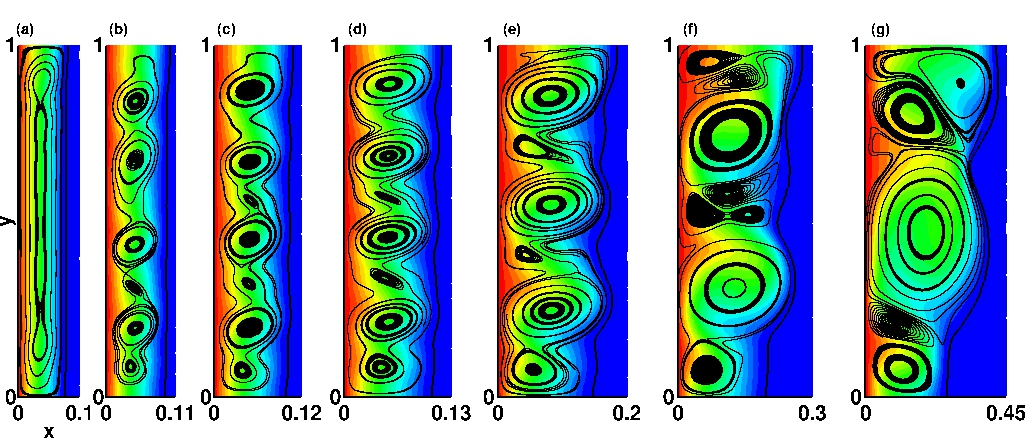
\includegraphics[width=\textwidth]{\figpath/Fig_cap_melting/evol_Gallium_FIELD}
		\end{minipage}
	\end{center}
	\caption{Case $\#4$ Melting of gallium: temperature field, streamlines, and melting front. 
	Physical time instants (panels a to g): $20 s$, $32s$, $36s$, $42s$, $85s$, $155s$, and $280s$.} \label{fig-Gallium}
\end{figure}

The time evolution of the flow is presented in the Figure \ref{fig-Gallium} with the plot of the streamlines for several physical times: $t_{\varphi} = 20s$, $32s$, $36s$, $42s$, $85s$, $155s$ and $280s$.
These times was voluntarily chosen for they correspond to roll merging.
\cite{hannoun2003resolving}, \cite{cerimele2002numerical} and \cite{giangi2000melting} compare the number of rolls in the fluid flow as a validation criterion.
Five primary cells are captured at $t=32s$ and decreases later through a process of roll merging as it is noticed by \cite{hannoun2003resolving}.
Our numerical results are in good agreement with the observations of \cite{hannoun2003resolving}, \cite{cerimele2002numerical} and \cite{giangi2000melting}.


